% Define the subtitle of the page
\title{Unsupervised learning}

% Begin the content of the page
\subsection{Unsupervised learning}

In unsupervised learning, the task is to infer hidden structure from
unlabeled data, comprised of training examples $\{x_n\}$.

We demonstrate how to do this in Edward with an example.
The script is available
\href{https://github.com/blei-lab/edward/blob/master/examples/mixture_gaussian.py}
{here}.


\subsubsection{Data}

Use a simulated dataset of 2-dimensional datapoints
$\mathbf{x}_n\in\mathbb{R}^2$.
\begin{lstlisting}[language=Python]
def build_toy_dataset(N):
    pi = np.array([0.4, 0.6])
    mus = [[1, 1], [-1, -1]]
    stds = [[0.1, 0.1], [0.1, 0.1]]
    x = np.zeros((N, 2), dtype=np.float32)
    for n in range(N):
        k = np.argmax(np.random.multinomial(1, pi))
        x[n, :] = np.random.multivariate_normal(mus[k], np.diag(stds[k]))

    return {'x': x}

data = build_toy_dataset(500)
\end{lstlisting}

We visualize the generated data points.
\begin{lstlisting}[language=Python]
plt.scatter(data['x'][:, 0], data['x'][:, 1])
plt.axis([-3, 3, -3, 3])
plt.show()
\end{lstlisting}
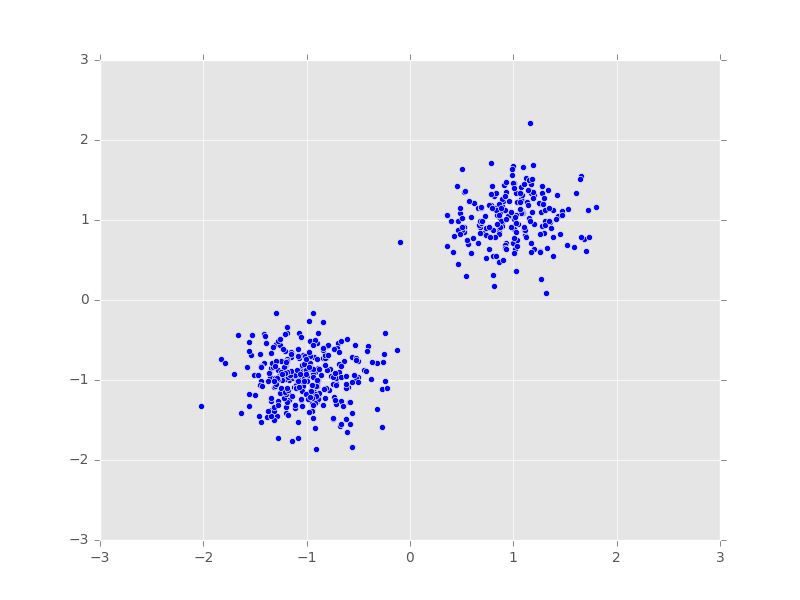
\includegraphics[width=700px]{images/unsupervised-fig0.png}

\subsubsection{Model}

Posit the model as a mixture of Gaussians. For more details on the
model, see the
\href{tut_mixture_gaussian.html}
{Mixture of Gaussians tutorial}.

Here we build the model in Edward using TensorFlow, and set the number
of mixture components to be 2.
\begin{lstlisting}[language=Python]
class MixtureGaussian:
    """
    Mixture of Gaussians

    p(x, z) = [ prod_{n=1}^N sum_{k=1}^K pi_k N(x_n; mu_k, sigma_k) ]
              [ prod_{k=1}^K N(mu_k; 0, cI) Inv-Gamma(sigma_k; a, b) ]
              Dirichlet(pi; alpha)

    where z = {pi, mu, sigma} and for known hyperparameters a, b, c, alpha.

    Parameters
    ----------
    K : int
        Number of mixture components.
    D : float, optional
        Dimension of the Gaussians.
    """
    def __init__(self, K, D):
        self.K = K
        self.D = D
        self.n_vars = (2*D + 1) * K

        self.a = 1
        self.b = 1
        self.c = 10
        self.alpha = tf.ones([K])

    def log_prob(self, xs, zs):
        """Return a vector [log p(xs, zs[1,:]), ..., log p(xs, zs[S,:])]."""
        x = xs['x']
        pi, mus, sigmas = zs
        log_prior = dirichlet.logpdf(pi, self.alpha)
        log_prior += tf.reduce_sum(norm.logpdf(mus, 0, np.sqrt(self.c)), 1)
        log_prior += tf.reduce_sum(invgamma.logpdf(sigmas, self.a, self.b), 1)

        # Loop over each sample zs[s, :].
        log_lik = []
        N = get_dims(x)[0]
        n_samples = get_dims(pi)[0]
        for s in range(n_samples):
            # log-likelihood is
            # sum_{n=1}^N log sum_{k=1}^K exp( log pi_k + log N(x_n; mu_k, sigma_k) )
            # Create a K x N matrix, whose entry (k, n) is
            # log pi_k + log N(x_n; mu_k, sigma_k).
            matrix = []
            for k in range(self.K):
                matrix += [tf.ones(N)*tf.log(pi[s, k]) +
                           multivariate_normal.logpdf(x,
                               mus[s, (k*self.D):((k+1)*self.D)],
                               sigmas[s, (k*self.D):((k+1)*self.D)])]

            matrix = tf.pack(matrix)
            # log_sum_exp() along the rows is a vector, whose nth
            # element is the log-likelihood of data point x_n.
            vector = log_sum_exp(matrix, 0)
            # Sum over data points to get the full log-likelihood.
            log_lik_z = tf.reduce_sum(vector)
            log_lik += [log_lik_z]

        return log_prior + tf.pack(log_lik)

model = MixtureGaussian(K=2, D=2)
\end{lstlisting}


\subsubsection{Inference}
Perform variational inference.
%
The latent variables are the mixture probabilities,
component means, and component variances.
Define the variational model to be a Dirichlet $\times$ fully factorized normal
$\times$ fully factorized inverse Gamma.
%The latent variables are $\mathbf{z} = (\pi, \mu, \sigma)$.
%\begin{align*}
%  q(\mathbf{z} \;;\; \lambda)
%  &=
%  \text{Dirichlet}(\mathbf{z}_\pi)
%  \times
%  \mathcal{N}(\mathbf{z}_\mu)
%  \times
%  \text{InvGamma}(\mathbf{z}_\sigma)
%\end{align*}
%
%The model in Edward is
\begin{lstlisting}[language=Python]
variational = Variational()
variational.add(Dirichlet(model.K))
variational.add(Normal(model.K*model.D))
variational.add(InvGamma(model.K*model.D))
\end{lstlisting}

Run mean-field variational inference for 4000 iterations, using a batch
of 10 datapoints and 50 latent variable samples per iteration.
\begin{lstlisting}[language=Python]
inference = ed.MFVI(model, variational, data)
inference.run(n_iter=4000, n_samples=50, n_minibatch=10)
\end{lstlisting}
In this case
\texttt{MFVI} defaults to minimizing the
$\text{KL}(q\|p)$ divergence measure using the score function
gradient.
For more details on inference, see the \href{tut_KLqp.html}{$\text{KL}(q\|p)$ tutorial}.


\subsubsection{Criticism}

We visualize the predicted memberships of each data point.
We pick the cluster assignment which produces
the highest log-likelihood for each data point.
First we output a K x N matrix of log-likelihoods, per
per-cluster assignment $k$ and per data-point $\mathbf{x}_n$.

We do this by adding the \texttt{predict()} method in the
probability model.
\begin{lstlisting}[language=Python]
class MixtureGaussian:
    ...
    def predict(self, xs, zs):
        """Return matrix with log-likelihoods for each data point under each cluster,
        averaging over each set of latent variables z in zs."""
        x = xs['x']
        pi, mus, sigmas = zs
        pi = tf.reduce_mean(pi, 0)
        mus = tf.reduce_mean(mus, 0)
        sigmas = tf.reduce_mean(sigmas, 0)

        matrix = []
        for k in range(self.K):
            matrix += [multivariate_normal.logpdf(x,
                               mus[(k*self.D):((k+1)*self.D)],
                               sigmas[(k*self.D):((k+1)*self.D)])]

        return tf.pack(matrix)
\end{lstlisting}
Then we evaluate the log-likelihood on the training data
and take the $\arg\max$ along the rows.
\begin{lstlisting}[language=Python]
clusters = np.argmax(ed.evaluate('log_likelihood', model, variational, data), axis=0)
\end{lstlisting}

Plot the data points, colored by their predicted membership.
\begin{lstlisting}[language=Python]
plt.scatter(data['x'][:, 0], data['x'][:, 1], c=clusters, cmap=cm.bwr)
plt.axis([-3, 3, -3, 3])
plt.show()
\end{lstlisting}

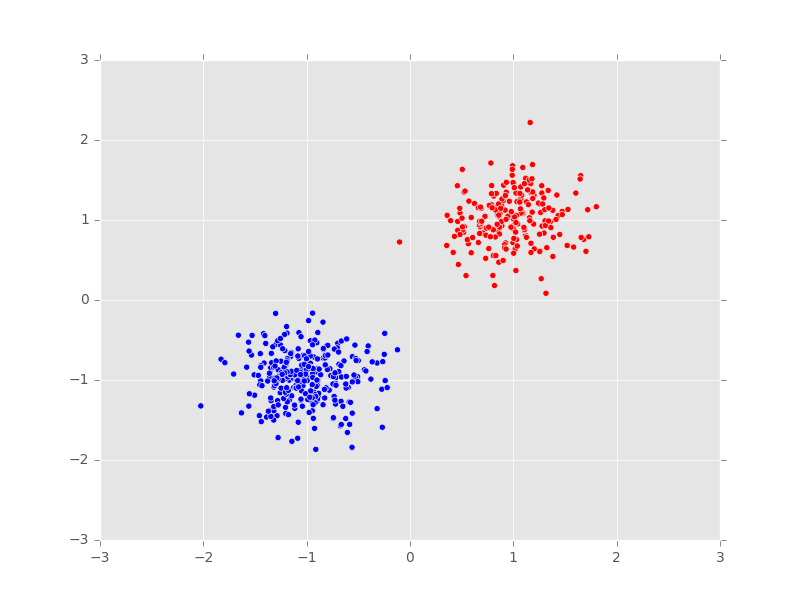
\includegraphics[width=700px]{images/unsupervised-fig1.png}
